\documentclass[11pt]{article}

%==Preamble================================================================================
\usepackage[dvipsnames, table]{xcolor}
\usepackage[utf8]{inputenc}

%==============================
\usepackage{amsmath}
\usepackage{amssymb}
\usepackage{stmaryrd}
\usepackage{mathtools}

%==============================
\usepackage[a4paper, margin=3cm]{geometry}
\usepackage[nodisplayskipstretch]{setspace}

\newcommand{\setStretchIndentAndSkip}{
  \setstretch{1.15}
%   \setlength\parindent{0pt}
  \setlength\parskip{12.5pt}
}

\usepackage[shortlabels]{enumitem}
\setlist{nosep}

\usepackage{titlesec}
\titlespacing{\paragraph}{%
  0pt}{%              left margin
  0pt}{  % space before (vertical)
  1em} % space after  (horizontal)

%==============================
\usepackage{tikz}
\usetikzlibrary{automata,calc,backgrounds,arrows.meta,decorations.pathmorphing,positioning}


\usepackage{tikz-cd}
\usepackage{quiver}

%==MACRO=====================================================
\newcommand{\A}{\mathbb{A}}
\newcommand{\N}{\mathbb{N}} % naturals / names / equality atoms
\newcommand{\Q}{\mathbb{Q}} % rationals / ordered atoms
\newcommand{\G}{\mathbb{G}} % Rado graph 
\newcommand{\V}{\mathbb{V}} % bit vectors
\newcommand{\W}{\mathbb{W}} % symplectic --- w for omega, or « double v » for the vector pair e, f

\newcommand{\FF}{\mathsf{F}} % field
\newcommand{\ff}{\mathsf{f}} % finite field
\newcommand{\EE}{\mathsf{E}} % abelian group

\newcommand{\Aut}{\operatorname{Aut}}
\newcommand{\Lin}{\operatorname{Lin}}
\newcommand{\len}{\operatorname{len}}
\newcommand{\Ker}{\operatorname{Ker}}
\newcommand{\Cog}{\operatorname{Cog}}
\newcommand{\supp}{\operatorname{supp}}

\DeclarePairedDelimiter\abs{\lvert}{\rvert}

\let\originalleft\left
\let\originalright\right
\renewcommand{\left}{\mathopen{}\mathclose\bgroup\originalleft}
\renewcommand{\right}{\aftergroup\egroup\originalright}


%==THEOREMS==================================================
\usepackage[hyperfootnotes=false]{hyperref}
\hypersetup{
    colorlinks = true,
    citecolor = magenta,
    linkcolor = .,
}
% !!!  !!!  !!!  !!!  !!! 
\usepackage{chngcntr}
% \counterwithout{equation}{section}
% \numberwithin{equation}{section}

\usepackage{aliascnt}

\renewcommand{\sectionautorefname}{Section}
%\renewcommand{\subtionautorefname}{Subsection}
%--
\usepackage{latexsym}
\usepackage[amsmath,thmmarks,framed]{ntheorem} 

\usepackage[ntheorem,framemethod=TikZ]{mdframed}

\mdfsetup{%
topline=false,
rightline=false,
bottomline=false,
linewidth=3pt,
innerleftmargin=15pt,
innerrightmargin=0pt,
skipabove=\baselineskip,
%skipbelow=\baselineskip,
}

\theoremstyle{break}

\newaliascnt{ThmCntr}{equation}
\newmdtheoremenv[linecolor=Black]{Thm}[ThmCntr]{Theorem}
\aliascntresetthe{ThmCntr}
\providecommand*{\ThmCntrautorefname}{Theorem}

\newaliascnt{QuestCntr}{equation}
\newmdtheoremenv[linecolor=BrickRed]{Quest}[QuestCntr]{Question}
\aliascntresetthe{QuestCntr}
\providecommand*{\QuestCntrautorefname}{Question}

\theoremstyle{plain}

\newaliascnt{CorCntr}{equation}
\newmdtheoremenv[linecolor=Black]{Cor}[CorCntr]{Corollary}
\aliascntresetthe{CorCntr}
\providecommand*{\CorCntrautorefname}{Corollary}

\newaliascnt{PropCntr}{equation}
\newmdtheoremenv[linecolor=Gray]{Prop}[PropCntr]{Proposition}
\aliascntresetthe{PropCntr}
\providecommand*{\PropCntrautorefname}{Proposition}

\newaliascnt{LemCntr}{equation}
\newmdtheoremenv[linecolor=Gray]{Lem}[LemCntr]{Lemma}
\aliascntresetthe{LemCntr}
\providecommand*{\LemCntrautorefname}{Lemma}

%--
\theorembodyfont{\upshape}

\theoremstyle{break}

\newaliascnt{DefCntr}{equation}
\newmdtheoremenv[linecolor=MidnightBlue]{Def}[DefCntr]{Definition}
\aliascntresetthe{DefCntr}
\providecommand*{\DefCntrautorefname}{Definition}


\theoremstyle{plain}

\newaliascnt{RqCntr}{equation}
\newmdtheoremenv[linecolor=MidnightBlue]{Rq}[RqCntr]{Remark}
\aliascntresetthe{RqCntr}
\providecommand*{\RqCntrautorefname}{Remark}

\newaliascnt{ExCntr}{equation}
\newmdtheoremenv[linecolor=MidnightBlue]{Ex}[ExCntr]{Example}
\aliascntresetthe{ExCntr}
\providecommand*{\ExCntrautorefname}{Example}


%--
\theoremstyle{nonumberplain}

\theoremheaderfont{\sc}
\theorembodyfont{\upshape\color{gray}}
\theoremseparator{.}
\theoremsymbol{\rule{1ex}{1ex}}
\newtheorem{Proof}{Proof}

%----
\usepackage[many]{tcolorbox}
\tcbuselibrary{skins,theorems}
\tcbset{
    before skip=\medskipamount,after skip=\bigskipamount,
}
\newtcolorbox{exo}[1][]{
    box align=top,
    title={#1},
    enhanced,
    parbox=false,
    colback=white, 
    colframe=MidnightBlue,
    coltitle=MidnightBlue,
    fonttitle=\bfseries,
    breakable,
    sharp corners,
    attach boxed title to top left={
        xshift=2ex,
        yshift=-4mm,
        yshifttext=-1mm,
    },
    boxed title style={
        colframe=white,
        colback=white,
    },
}

%\NewTcbTheorem[
%    use counter=equation,
%    number within=subsection,
%]{Def}{Definition}{
%    colback=white,
%    colframe=Black,
%    fonttitle=\bfseries,
%    enhanced,
%    breakable,
%    sharp corners,
%    coltitle=Black,
%    attach boxed title to top left={
%        xshift=2ex,
%        yshift=-4mm,
%        yshifttext=-1mm,
%    },
%    boxed title style={
%        colframe=white,
%        colback=white,
%    }
%}{Def}





%==========================================================================================
% \usepackage{gfsdidot}
% \usepackage[bigdelims]{newtxmath}
% \usepackage{eucal}

% \usepackage{anyfontsize}

\usepackage{nicematrix}
\usepackage{cancel}

\usepackage[T2A,T1]{fontenc}

\newcommand{\Che}{K}
\newcommand{\Tse}{V'}
\newcommand{\Sha}{V}

\usepackage[symbol]{footmisc}

\def\amalgindep{\mathrel{\raise0.2ex\hbox{\ooalign{\hidewidth$\vert$\hidewidth\cr\raise-0.9ex\hbox{$\smile$}}}}}


%==========================================================================================



\begin{document}

\title{Cogs span the projection kernel, version $n+1$}
\author{Jingjie Yang}
% \date{}

\maketitle
\setStretchIndentAndSkip
\allowdisplaybreaks

\section{Notations}
Let $\mathcal{O} \subseteq \A^I$ be an $S$-ordered orbit.
Given a vector $v \in \Lin_\EE \mathcal{O}$, write $\underline{v}$ for its set-theoretic support, i.e., the finite subset $v^{-1}(\EE^*) \subseteq \mathcal{O}$.
More generally, given any finite subset $\sigma \subseteq \mathcal{O}$, 
write
\[
    \overline{\sigma} = \{ (i, a_i) \mid i \in I, a \in \sigma \}
\]
and define two binary relations 
\begin{align*}
    &(i, a_i) {?} (j, b_j) \iff a_i = b_j \text{ but } i \neq j, \\
    &(i, a_i) {!} (j, b_j) \iff \text{$a_i, b_j$ are related but not in the same way as $a_i, a_j$}
    % or equivalently $b_i, b_j$ since both $a$ and $b$ are in $\mathcal{O}$
\end{align*}
called \emph{ambiguities} and \emph{obstructions}.
(Recall that $a_i$ and $b_j$ are \emph{not related} if they are freely amalgamated in the reduct $\A_0$ of $\A$ 
--- i.e., they are not equal, and for no $R \in \mathcal{L}_0$ does $R(a_i, b_j) \vee R(b_j, a_i)$ hold;
in that case, we write $a_i \amalgindep b_j$).
Both relations are symmetric and ${?} \subseteq {!}$;
denote their images by ${?\overline{\sigma}} \subseteq {!\overline{\sigma}} \subseteq \overline{\sigma}$.
Lastly, refer to the atoms that appear in $\sigma$ by $\sqrt \sigma \subseteq \A$.
\begin{Rq}\label{Rq:unambiguous}
    Assume $?\overline{\sigma} = \emptyset$.
    Given any $a_i \in \sqrt{\sigma}$, we have $(i, a_i) \in \overline{\sigma}$.
\end{Rq}

The prototypical example of an unobstructed family is $\overline{\underline{\lambda \cdot a^+ \between a^-}} = \overline{\{a^+, a^-\}} = \overline{\{a^\pm\}}$,
where $a^+ \parallel a^-$ is an $\mathcal{O}$-dipole.

\section{Lemmas}
Let $v \in \Ker_\EE \mathcal{O}$ and let $v^{i:a_i}$ be a subvector.
In the cog decomposition results we are about to prove,
we will work with the assumption that $\Sha = \underline{v}$ is unobstructed (resp., unambiguous);
then so is $\Tse = \underline{v^{i:a_i}} \subseteq \underline{v}$.
We will be able to write $v^{i:a_i} = \sum_{a^\pm \in A^\pm} (\lambda_{a^\pm} \cdot a^+ \between a^-) a_i$
where the union of $\Tse$ and $\Che = A^\pm a_i = \{a^+ a_i, a^- a_i \mid a^\pm \in A^\pm\}$ is unobstructed (resp., unambiguous).
But we want to make $\Sha \cup \Che$ unobstructed (resp., unambiguous);
we can do so by choosing $\Che$ more carefully.

% Here O is orbit of edges (a, b) with a < b, a ~ b.
% The YELLOW family of edges, which contains the GREEN family, has no obstructions.
% Nor does the union of GREEN and RED. 
% However YELLOW and RED together has an ambiguity (2, b) ? (1, b).
% Lemma-? removes ambiguities but still leaves an obstruction (2, \pi b) ! (2, d).
% Lemma-! removes such obstructions.
\begin{center}
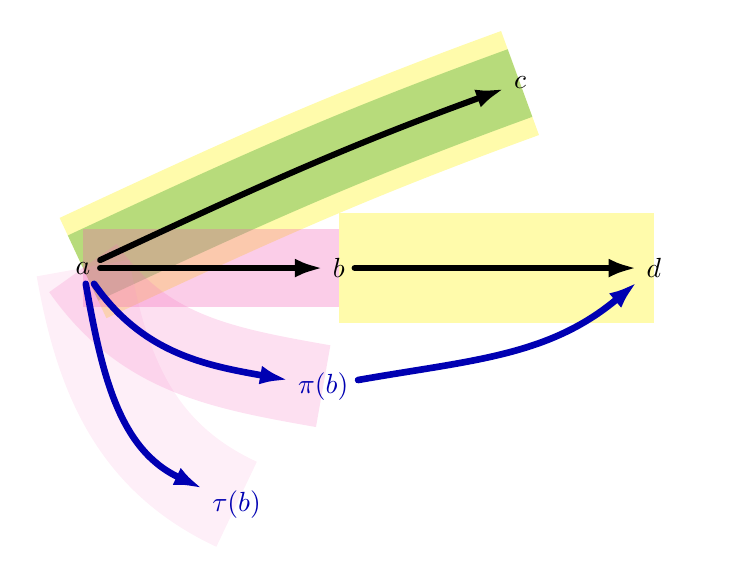
\begin{tikzpicture}[font=\sffamily, line cap=round, line join=round, >={Latex[length=3.6mm,width=2.4mm]}]
\coordinate (a) at (0,0); \coordinate (b) at (3.25,0); \coordinate (d) at (7.25,0); \coordinate (c) at (5.55,2.35); \coordinate (pib) at (3.05,-1.5); \coordinate (taub) at (1.95,-3);
\begin{scope}[on background layer]
\draw[yellow!60, opacity=0.55, line width=40pt] (a) to[out=25,in=200] (c); \draw[green!55!black, opacity=0.28, line width=26pt] (a) to[out=25,in=200] (c);
\draw[yellow!60, opacity=0.55, line width=40pt] (b) -- (d);
\draw[magenta!65, opacity=0.30, line width=28pt] (a) -- (b);
\draw[magenta!55, opacity=0.22, line width=30pt] (a) to[out=-55,in=170] (pib);
\draw[magenta!45, opacity=0.14, line width=34pt] (a) to[out=-80,in=155] (taub);    
\end{scope}
\node (A) at (a) {$a$}; \node (B) at (b) {$b$}; \node (C) at (c) {$c$}; \node (D) at (d) {$d$}; \node[blue!70!black] (PIB) at (pib) {$\pi(b)$}; \node[blue!70!black] (TAUB) at (taub) {$\tau(b)$};
\draw[->, line width=2.2pt] (A) to[out=25,in=200] (C);
\draw[->, line width=2.2pt] (A) -- (B);
\draw[->, line width=2.2pt] (B) -- (D);
\draw[->, line width=2.4pt, blue!70!black] (A) to[out=-55,in=170] (PIB);
\draw[->, line width=2.4pt, blue!70!black] (A) to[out=-80,in=155] (TAUB);
\draw[->, line width=2.4pt, blue!70!black] (PIB) to[out=10,in=-140] (D);
\end{tikzpicture}
\end{center}

\begin{Lem}\label{lem:?}
    Let $\Che, \Tse, \Sha$ be finite subsets of $\mathcal{O}$ such that ${?}\overline{\Tse \cup \Che} = \emptyset = {?}\overline{\Sha} \supseteq {?}\overline{\Tse}$.
    Then there exists $\pi \in \Aut(\A / S \cup \sqrt{\Tse})$ that satisfies
    \[
        ?\overline{\Sha \cup \pi(\Che)} = \emptyset.
    \]
\end{Lem}
\begin{Proof}
    Fix $\Tse, \Sha$ and induct on the size of $? \overline{\Sha \cup \Che}$.
    
    Let $(i, a_i) ? (j, b_j)$; without loss of generality we may assume $(j, b_j) \in \overline{\Sha}$ and $(i, a_i) \in \overline{\Che} \setminus \overline{\Tse}$.
    Since $?\overline{\Tse} = \emptyset$, by \autoref{Rq:unambiguous} we see that $a_i \not\in \sqrt{\Tse}$; also $a_i \not\in S$, as $\mathcal{O}$ is $S$-ordered.
    With strong amalgamation, we may find some $\pi \in \Aut(\A / S \cup \sqrt{\Tse})$ such that $\pi(a_i) \not\in \sqrt{\Sha \cup \Che}$.
    Now it is straightforward to check that
    \[
        {?}\overline{\Sha \cup \pi(\Che)} \subseteq {?}\overline{\Sha \cup \Che} \setminus \{(i, a_i)\}.
    \]
    Because ${?}\overline{\Tse \cup \pi(\Che)} = {?}\overline{\pi(\Tse) \cup \pi(\Che)} = \pi(\emptyset) = \emptyset$ still,
    the inductive hypothesis gives us some $\pi' \in \Aut(\A / S \cup \sqrt{\Tse})$ such that $?\overline{\Sha \cup \pi' \pi(\Che)} = \emptyset$.
\end{Proof}

\begin{Lem}\label{lem:!}
    Let $\Che, \Tse, \Sha$ be finite subsets of $\mathcal{O}$ such that $!\overline{\Tse \cup \Che} = \emptyset = {!}\overline{\Sha} \supseteq {!}\overline{\Tse}$.
    Then
    \[
        !\overline{\Sha \cup \pi(\Che)} = \emptyset
    \]
    for some $\pi \in \Aut(\A / S \cup \sqrt{\Tse})$.
\end{Lem}
\begin{Proof}
    By \autoref{lem:?} we may assume that $?\overline{\Sha \cup \Che} = \emptyset$ already.
    As before, fix $\Tse, \Sha$ and proceed by induction on the size of $!\overline{\Sha \cup \Che}$.
    
    Let $(i, a_i) ! (j, b_j)$; without loss of generality we may assume $(j, b_j) \in \overline{\Sha}$ and $(i, a_i) \in \overline{\Che}$.
    Now $(i, a_i) \not\in \overline{\Tse}$, so $a_i \not\in \sqrt{\Tse}$ by \autoref{Rq:unambiguous};
    further, whenever $(i, a_i) ! (k, c_k)$ we observe that $c_k \not\in S \cup \{a_i\} \cup \sqrt{\Che \cup \Tse}$.
    Let $Y$ consist of all such $c_k$ and put
    \[
        X = S \cup \sqrt{\Che \cup \Sha} \setminus (Y \cup \{a_i\}).
    \]
    Then $X, Y, \{a_i\}$ are pairwise disjoint, and we see $X$ contains $S \cup \sqrt{\Tse}$ as well as $\sqrt{\Che} \setminus \{a_i\}$.
    With free amalgamation (in $\A_0$) this time, we may find some $\tau \in \Aut(\A / S \cup \sqrt{\Tse})$ such that $\tau(a_i) \not\in X \cup Y \cup \{a_i\}$ and $\tau \amalgindep Y$. 
    Again, we can check that
    \[
        {!}\overline{\Sha \cup \tau(\Che)} \subseteq {!}\overline{\Sha \cup \Che} \setminus (i, a_i)
    \]
    so the conclusion follows straightforwardly from the inductive hypothesis.
\end{Proof}

\section{Unobstructed vector}
% https://q.uiver.app/#q=WzAsMTUsWzAsMywiYl4rIl0sWzEsMywiYiJdLFswLDQsImJeLSJdLFswLDAsImFeKyJdLFsxLDEsImEiXSxbMCwxLCJhXi0iXSxbMywyLCJjIl0sWzQsMiwiXFxyaWdodHNxdWlnYXJyb3ciXSxbNSwzLCJiXisiXSxbNSw0LCJiXi0iXSxbNSwxLCJhXi0iXSxbNSwwLCJhXisiXSxbNiwxLCJhIl0sWzYsMywiYiJdLFs4LDIsImMiXSxbMCwxLCIiLDAseyJjb2xvdXIiOlswLDYwLDYwXX1dLFsyLDEsIiIsMix7ImNvbG91ciI6WzI0MCw2MCw2MF19XSxbMyw0LCIiLDIseyJjb2xvdXIiOlswLDYwLDYwXX1dLFs1LDQsIiIsMCx7ImNvbG91ciI6WzI0MCw2MCw2MF19XSxbMyw2LCIiLDAseyJjdXJ2ZSI6LTF9XSxbNSw2XSxbMCw2XSxbMiw2LCIiLDIseyJjdXJ2ZSI6MX1dLFsxMCwxNCwiIiwwLHsiY29sb3VyIjpbMjQwLDYwLDYwXX1dLFs4LDE0LCIiLDIseyJjb2xvdXIiOlswLDYwLDYwXX1dLFs4LDEzXSxbOSwxM10sWzExLDEyXSxbMTAsMTJdLFsxMSwxNCwiIiwxLHsiY3VydmUiOi0xLCJjb2xvdXIiOlswLDYwLDYwXX1dLFs5LDE0LCIiLDEseyJjdXJ2ZSI6MSwiY29sb3VyIjpbMjQwLDYwLDYwXX1dXQ==
\[\begin{tikzcd}[cramped]
	{a^+} &&&&& {a^+} \\
	{a^-} & a &&&& {a^-} & a \\
	&&& c & \rightsquigarrow &&&& c \\
	{b^+} & b &&&& {b^+} & b \\
	{b^-} &&&&& {b^-}
	\arrow[draw={rgb,255:red,214;green,92;blue,92}, from=1-1, to=2-2]
	\arrow[curve={height=-6pt}, from=1-1, to=3-4]
	\arrow[from=1-6, to=2-7]
	\arrow[color={rgb,255:red,214;green,92;blue,92}, curve={height=-6pt}, from=1-6, to=3-9]
	\arrow[draw={rgb,255:red,92;green,92;blue,214}, from=2-1, to=2-2]
	\arrow[from=2-1, to=3-4]
	\arrow[from=2-6, to=2-7]
	\arrow[color={rgb,255:red,92;green,92;blue,214}, from=2-6, to=3-9]
	\arrow[from=4-1, to=3-4]
	\arrow[draw={rgb,255:red,214;green,92;blue,92}, from=4-1, to=4-2]
	\arrow[color={rgb,255:red,214;green,92;blue,92}, from=4-6, to=3-9]
	\arrow[from=4-6, to=4-7]
	\arrow[curve={height=6pt}, from=5-1, to=3-4]
	\arrow[draw={rgb,255:red,92;green,92;blue,214}, from=5-1, to=4-2]
	\arrow[color={rgb,255:red,92;green,92;blue,214}, curve={height=6pt}, from=5-6, to=3-9]
	\arrow[from=5-6, to=4-7]
\end{tikzcd}\]
\begin{Prop}\label{prop:!-free-decomposition}
    \footnote[0]{This is the same statement as in \S{}IV.D; here I use a slightly different proof.}
    Let $v \in \Ker_\EE \mathcal{O}$ and suppose that $!\overline{\underline v} = \emptyset$.
    Then we can write
    \[
        v = \sum_{a^\pm \in A^\pm} \lambda_{a^\pm} \cdot a^+ \between a^-
    \]
    with $!\overline{\underline{v} \cup A^\pm} = \emptyset$ and $\lambda_{a^\pm} \in v(\mathcal{O})$.
\end{Prop}

We proceed by induction on the dimension $|I|$, 
noting that when $I = \emptyset$ we just have $v = v() \cdot () = v() \cdot ( \between )$ without any possible obstructions.

So suppose $I$ is non-empty; let $d \in I$ be the greatest. 
Group the terms in $v$ by their greatest atom so that $v = v^1 + v^2 + \cdots + v^k$.
We now induct on $k$.
If $k < 2$, we are done: as $v_{-d} = 0$ we must have $v = 0$, so the empty sum will do.
Otherwise \[
    v = v^{d:a_d} + v^{d:b_d} + v'.
\]
By the outer inductive hypothesis, we get \[
    v^{d:a_d} = v^{d:a_d}_{-d} a_d = \sum_{A^\pm} (\lambda_{a^\pm} \cdot a^+ \between a^-)a_d
\]
where we only know $!\overline{\underline{v^{d:a_d}_{-d}} \cup A^\pm} = \emptyset$ so that $!\overline{\underline{v^{d:a_d}} \cup A^\pm a_d} = \emptyset$.
But any $\pi \in \Aut(\A / S \cup \sqrt{\underline{v^{d:a_d}}})$ satisfies 
\[
    v^{d:a_d} = \pi(v^{d:a_d}) = \sum_{a^\pm \in A^\pm} \lambda_{a^\pm} \cdot \pi a^+ \between \pi a^-,
\]
so by \autoref{lem:!} we may assume without loss of generality that \[
    !\overline{\underline{v} \cup A^\pm a_d} = \emptyset.
\]
Similarly, we can write \[
    v^{d:a_d} = \sum_{B^\pm} (\lambda_{b^\pm} \cdot b^+ \between b^-)b_d
\]
where, in turn, we may upgrade the assumption that $! \overline{\underline{v^{d:b_d}} \cup B^\pm b_d} = \emptyset$ to \[
    !\overline{\underline{v} \cup A^\pm a_d \cup B^\pm b_d} = \emptyset.
\]

The key is that we may now invent a new element $z$, on which we impose the following relations with $S \cup \sqrt{A^\pm a_d \cup B^\pm b_d} \subseteq \A$: 
\begin{enumerate}
    \item $a_d, b_d < z$, and $z < s$ if $a_d, b_d < s$ for some $s \in S$ (enough to let $s$ be the least such);
    
    \item for any unary relation $P \in \mathcal{L}_0$:
    \[
        P(z) \;:\Longleftrightarrow\; P(a_d) \iff P(b_d)
    \]
    --- recall that $a, b \in \mathcal{O}$;
    \item for any binary relation $R \in \mathcal{L}_0$ and $s \in S$, $a^\pm \in A^\pm$, $b^\pm \in B^\pm$, $i \in I \setminus \{d\}$:
    \begin{enumerate}
        \item $R(z, s) \;:\Longleftrightarrow\; R(a_d, s) \iff R(b_d, s)$,
        % \item $R(s, z) \;:\Longleftrightarrow\; R(s, a_d) \iff R(s, b_d)$;
        \item $R(z, a^\pm_i) \;:\Longleftrightarrow\; R(a_d, a^\pm_i)$,
        \item $R(z, a_d) \;:\Longleftrightarrow\; \bot$,
        \item $R(z, b^\pm_i) \;:\Longleftrightarrow\; R(b_d, b^\pm_i)$;
        % \item $R(c_i, z) \;:\Longleftrightarrow\; R(c_i, a_d) \iff R(c_i, b_d)$;
        \item $R(z, b_d) \;:\Longleftrightarrow\; \bot$,
        % \item $R(a_d, z), R(b_d, z) \;:\Longleftrightarrow\; \bot$;
        \item and symmetrically for $R(-, z)$.
    \end{enumerate}
    These are well-defined because $a^\pm a_d, b^\pm b_d \in \mathcal{O}$ and $i = j$ whenever $a^\pm_i = b^\pm_j$.
\end{enumerate}
To see that the $\mathcal{L}$-structure $S \cup \sqrt{A^\pm a_d \cup B^\pm b_d} \cup \{z\}$ still embeds into $\A$, 
suppose towards a contradiction that it contains a forbidden $\mathcal{L}_0$-substructure $F$.
Then $F$ must contain $z$.
Since any two elements in $F$ are necessarily related, we must have $a_d, b_d \not\in F$.
Similarly, whenever $F$ contains $x_i$ where $x \in A^\pm \cup B^\pm, i \in I \setminus \{d\}$ it does not contain a distinct atom of the form $x'_i$.
It follows that \[
    s \mapsto s,\quad x_i \mapsto a_i,\quad z \mapsto a_d
\]
defines an injective function $\phi : F \to \A_0$,
which is furthermore an embedding (we only need to check this for pairs!) because $!\overline{A^\pm \cup B^\pm} = \emptyset$ and any $x_i, x'_{i'}$ for $i \neq i'$ are related.
This is impossible --- therefore assume $z \in \A$.

It is now routine to check that $a^+ a_d \parallel a^- z$ and $b^+ a_d \parallel b^- z$ are $\mathcal{O}$-dipoles for $a^\pm \in A^\pm, b^\pm \in B^\pm$
and that $!\overline{A^+ a_d \cup A^- z \cup B^+ b_d \cup B^- z} = \emptyset$.
By \autoref{lem:!} we may assume %since $!\overline{\underline{v} \cup A^\pm a_d \cup B^\pm b_d}$ is empty
that $!\overline{\underline{v} \cup A^+ a_d \cup A^- z \cup B^+ b_d \cup B^- z} = \emptyset$. 
(Alternatively, we could have explicitly ensured this when defining $z$).
Then
\begin{align*}
    v'' &= v
    - \sum_{A^\pm} \lambda_{a^\pm} \cdot a^+ a_d \between a^- z 
    - \sum_{B^\pm} \lambda_{b^\pm} \cdot b^+ b_d \between b^- z  \\
    &= v^{d:a_d}_{-d} z + v^{d:b_d}_{-d} z + v',
\end{align*}
when grouped into subvectors by the largest atom in each term, has at least one fewer component than $v$.
By the inner inductive hypothesis, we may write
we may write 
\[
    v'' = \sum_{C^\pm} \lambda_{c^\pm} \cdot c^+ \between c^-
\]
where $!\overline{\underline{v''} \cup C^\pm} = \emptyset$.
But $\overline{\underline{v''}} \subseteq \overline{\underline{v} \cup A^+ a_d \cup A^- z \cup B^+ b_d \cup B^- z}$, 
so one last application of \autoref{lem:!} allows us to assume that
\[
    !\overline{\underline{v} \cup A^+ a_d \cup A^- z \cup B^+ b_d \cup B^- z \cup C^\pm} = \emptyset.
\]
We conclude that
\[
    v = 
      \sum_{A^\pm} \lambda_{a^\pm} \cdot a^+ a_d \between a^- z 
    + \sum_{B^\pm} \lambda_{b^\pm} \cdot b^+ b_d \between b^- z
    + \sum_{C^\pm} \lambda_{c^\pm} \cdot c^+ \between c^-;
\]
in other words, we have decomposed an unobstructed vector into an unobstructed family of cogs.
\textcolor{red}{(The notation $\lambda_{a^\pm}, \lambda_{b^\pm}$ is a bit sloppy ...)}


\section{Unambiguous vector}
% https://q.uiver.app/#q=WzAsMTUsWzAsMSwiYSJdLFsyLDAsImIiXSxbMiwyLCJjIl0sWzEsMSwiYSciXSxbMSwzLCJkIl0sWzIsMywiZSJdLFsyLDQsImYiXSxbMywyLCJcXHJpZ2h0c3F1aWdhcnJvdyJdLFs0LDEsImEiXSxbNSwxLCJhJyJdLFs2LDAsImIiXSxbNiwyLCJjIl0sWzUsMywiZCJdLFs2LDMsImUiXSxbNiw0LCJmIl0sWzAsMSwiIiwyLHsiY29sb3VyIjpbMCw2MCw2MF19XSxbMCwyLCIiLDAseyJjb2xvdXIiOlsyNDAsNjAsNjBdfV0sWzMsMV0sWzMsMl0sWzQsNSwiIiwwLHsiY29sb3VyIjpbMCw2MCw2MF19XSxbNCw2LCIiLDIseyJjb2xvdXIiOlsyNDAsNjAsNjBdfV0sWzAsNF0sWzgsMTBdLFs5LDEwLCIiLDIseyJjb2xvdXIiOlswLDYwLDYwXX1dLFs5LDExLCIiLDAseyJjb2xvdXIiOlsyNDAsNjAsNjBdfV0sWzgsMTJdLFsxMiwxMywiIiwyLHsiY29sb3VyIjpbMCw2MCw2MF19XSxbMTIsMTQsIiIsMix7ImNvbG91ciI6WzI0MCw2MCw2MF19XSxbOCwxMV1d
\[\begin{tikzcd}[cramped]
	&& b &&&& b \\
	a & {a'} &&& a & {a'} \\
	&& c & \rightsquigarrow &&& c \\
	& d & e &&& d & e \\
	&& f &&&& f
	\arrow[color={rgb,255:red,214;green,92;blue,92}, from=2-1, to=1-3]
	\arrow[color={rgb,255:red,92;green,92;blue,214}, from=2-1, to=3-3]
	\arrow[from=2-1, to=4-2]
	\arrow[from=2-2, to=1-3]
	\arrow[from=2-2, to=3-3]
	\arrow[from=2-5, to=1-7]
	\arrow[from=2-5, to=3-7]
	\arrow[from=2-5, to=4-6]
	\arrow[color={rgb,255:red,214;green,92;blue,92}, from=2-6, to=1-7]
	\arrow[color={rgb,255:red,92;green,92;blue,214}, from=2-6, to=3-7]
	\arrow[color={rgb,255:red,214;green,92;blue,92}, from=4-2, to=4-3]
	\arrow[color={rgb,255:red,92;green,92;blue,214}, from=4-2, to=5-3]
	\arrow[color={rgb,255:red,214;green,92;blue,92}, from=4-6, to=4-7]
	\arrow[color={rgb,255:red,92;green,92;blue,214}, from=4-6, to=5-7]
\end{tikzcd}\]
\begin{Prop}\label{prop:?-free-decomposition}
    \footnote[0]{This is an amended version of Proposition~IV.25 (the one with $\acute{\ddot v}$). The proof there had a gap, which is filled by the additional conclusion about unambiguity here.}
    Let $v \in \Ker_\EE \mathcal{O}$ and suppose that $?\overline{\underline v} = \emptyset$.
    Then we can write
    \[
        v = \sum_{a^\pm \in A^\pm} \lambda_{a^\pm} \cdot a^+ \between a^-
    \]
    with $?\overline{\underline{v} \cup A^\pm} = \emptyset$ and $\lambda_{a^\pm} \in v(\mathcal{O})$.
\end{Prop}
We proceed again by induction, first on the dimension $|I|$ then on the cardinality of $! \overline{\underline{v}}$.
The outer base case $I = \emptyset$ is trivial 
--- we have $v = v() \cdot ( \between )$, and no ambiguities may arise
--- whilst the inner base case is just \autoref{prop:!-free-decomposition}.

So suppose that $!\overline{\underline{v}}$ contains some $(i, a_i)$.
Since $\overline{\underline{v^{i:a_i}_{-i}}} \subseteq \overline{\underline{v^{i:a_i}}} \subseteq \overline{\underline{v}}$, we know that $v^{i:a_i}_{-i}$ is unambiguous.
Applying the outer inductive hypothesis, we may write
\[
    v^{i:a_i} = v^{i:a_i}_{-i} a_i = \sum_{A^\pm} (\lambda_{a^\pm} \cdot a^+ \between a^-) a_i
\]
where $\emptyset = ?\overline{(\underline{v^{i:a_i}_{-i}} \cup A^\pm) a_i} = ?\overline{\underline{v^{i:a_i}} \cup A^\pm a_i}$.
Moreover, we may assume by \autoref{lem:?} that \[
    ?\overline{\underline{v} \cup A^\pm a_i} = \emptyset.
\]
Now we can show that whenever $(j, b_j) ! (i, a_i)$ in $\overline{\underline{v}}$ we have $b_j \not\in \sqrt{A^\pm a_i}$.
Already $b_j = a_i$ would imply $j = i$ as $?\overline{\underline{v}} = 0$, which is impossible.
So suppose to the contrary that $b_j = a^\pm_k$ for some $a^\pm \in A^\pm$ and $k \in I \setminus \{i\}$.
By the assumption above, we must have $j = k$;
this is a contradiction: note that $a^\pm a_i \in \mathcal{O}$.

Put $Y = \{b_j \mid (j, b_j) \in \overline{\underline{v}}, (j, b_j) ! (i, a_i)\}$.
It follows that $X = S \cup \sqrt{\underline{v} \cup A^\pm} \setminus Y \setminus \{a_i\}$ contains $S \cup \sqrt{A^\pm}$ and that $X, Y, \{a_i\}$ are pairwise disjoint.
Using free amalgamation in $\A_0$, we may find $\tau \in \Aut(\A / X)$ such that $\tau(a_i) \not\in X \cup Y \cup \{a_i\}$, is greater than $a_i$, and is not related to any of $Y \cup \{a_i\}$.
Then, given any $a^\pm \in A^\pm$, we can straightforwardly check that $a^+ a_i \parallel a^- \tau(a_i)$ is an $\mathcal{O}$-dipole, 
that $?\overline{\underline{v} \cup A^+ a_i \cup A^- \tau(a_i)} = \emptyset$,
and that
\begin{align*}
    v - \sum_{A^\pm} \lambda_{a^\pm} \cdot a^+ a_i \between a^- \tau(a_i)
    &= v -  v^{i:a_i} + v^{i:\tau(a_i)}\\
    &= v^{i : a_i \mapsto \tau(a_i)}    
\end{align*}
satisfies ${!}\overline{\underline{v^{i : a_i \mapsto \tau(a_i)}}} \subseteq {!}\overline{\underline{v}} \setminus \{(i, a_i)\}$.
The inner inductive hypothesis tells us 
that $v^{i : a_i \mapsto \tau(a_i)} = \sum_{B^\pm} \lambda_{B^\pm} \cdot b^+ \between b^-$ 
with \[
    ?\overline{\underline{v^{i : a_i \mapsto \tau(a_i)}} \cup B^\pm} = \emptyset.
\]
But $\overline{\underline{v^{i : a_i \mapsto \tau(a_i)}}} \subseteq \overline{\underline{v} \subseteq A^+ a_i \cup A^- \tau(a_i)}$,
so \autoref{lem:?} allows us to assume that \[
    ? \overline{\underline{v} \cup A^+ a_i \cup A^- \tau(a_i) \cup B^\pm} = \emptyset.
\]
We conclude that 
\[
    v =\sum_{A^\pm} \lambda_{a^\pm} \cdot a^+ a_i \between a^- \tau(a_i) + \sum_{B^\pm} \lambda_{b^\pm} \cdot b^+ \between b^-
\]
--- in other words, we have decomposed an unambiguous vector into an unambiguous family of cogs.

\section{General vector}
% https://q.uiver.app/#q=WzAsMTMsWzAsMSwiXFxkb3RzIl0sWzEsMiwiYSJdLFswLDMsIlxcZG90cyJdLFszLDAsImIiXSxbMyw0LCJjIl0sWzIsMiwiYSciXSxbNCwyLCJcXHJpZ2h0c3F1aWdhcnJvdyJdLFs1LDEsIlxcY2RvdHMiXSxbNSwzLCJcXGNkb3RzIl0sWzYsMiwiYSJdLFs4LDAsImIiXSxbOCw0LCJjIl0sWzcsMiwiYSciXSxbMiwxLCIiLDIseyJjb2xvdXIiOlsyNDAsNjAsNjBdfV0sWzEsMywiIiwyLHsiY29sb3VyIjpbMCw2MCw2MF19XSxbMSw0LCIiLDIseyJjb2xvdXIiOlsyNDAsNjAsNjBdfV0sWzUsM10sWzUsNF0sWzAsMSwiIiwwLHsiY29sb3VyIjpbMCw2MCw2MF19XSxbNyw5LCIiLDIseyJjb2xvdXIiOlswLDYwLDYwXX1dLFs4LDksIiIsMCx7ImNvbG91ciI6WzI0MCw2MCw2MF19XSxbOSwxMF0sWzksMTFdLFsxMiwxMCwiIiwyLHsiY29sb3VyIjpbMCw2MCw2MF19XSxbMTIsMTEsIiIsMSx7ImNvbG91ciI6WzI0MCw2MCw2MF19XV0=
\[\begin{tikzcd}[cramped]
	&&& b &&&&& b \\
	\dots &&&&& \cdots \\
	& a & {a'} && \rightsquigarrow && a & {a'} \\
	\dots &&&&& \cdots \\
	&&& c &&&&& c
	\arrow[color={rgb,255:red,214;green,92;blue,92}, from=2-1, to=3-2]
	\arrow[color={rgb,255:red,214;green,92;blue,92}, from=2-6, to=3-7]
	\arrow[color={rgb,255:red,214;green,92;blue,92}, from=3-2, to=1-4]
	\arrow[color={rgb,255:red,92;green,92;blue,214}, from=3-2, to=5-4]
	\arrow[from=3-3, to=1-4]
	\arrow[from=3-3, to=5-4]
	\arrow[from=3-7, to=1-9]
	\arrow[from=3-7, to=5-9]
	\arrow[color={rgb,255:red,214;green,92;blue,92}, from=3-8, to=1-9]
	\arrow[color={rgb,255:red,92;green,92;blue,214}, from=3-8, to=5-9]
	\arrow[color={rgb,255:red,92;green,92;blue,214}, from=4-1, to=3-2]
	\arrow[color={rgb,255:red,92;green,92;blue,214}, from=4-6, to=3-7]
\end{tikzcd}\]
\begin{Prop}
    \footnote[0]{This is the same statement and proof as Proposition~IV.24 (the one with $\ddot v$).}
    Let $v \in \Ker_\EE \mathcal{O}$.
    Then we can write
    \[
        v = \sum_{a^\pm \in A^\pm} \lambda_{a^\pm} \cdot a^+ \between a^-
    \]
    with $\lambda_{a^\pm} \in v(\mathcal{O})$.
\end{Prop}
This is an easier induction on $|I|$ then on $?\overline{\underline{v}}$.
If $I = \emptyset$, the decomposition is trivial; 
if $v$ is unambiguous already, the decomposition comes from \autoref{prop:?-free-decomposition}.

Now suppose $?\overline{\underline{v}}$ contains some $(i, a_i)$,
and use the outer inductive hypothesis to write 
\[
    v^{i:a_i}
    = v^{i:a_i}_{-i} a_i 
    = \sum_{A^\pm} (\lambda_{a^\pm} \cdot a^+ \between a^-) a_i.
\]
Then neither $S$ nor $\sqrt{A^\pm}$ contains $a_i$,
so $X = S \cup \sqrt{\underline{v} \cup A^\pm} \setminus \{a_i\}$ contains $S \cup \sqrt{A^\pm}$.
Using free amalgamation in $\A_0$ and the generic order in $\A$, we may find some $\pi \in \Aut(\A / X)$ such that 
$\pi(a_i) \not\in X$, 
$\pi(a_i) > a_i$, 
$\pi(a_i) \amalgindep a_i$. % This 'stationary independence relation' symbol means: 
% \pi(a_i) and a_i are freely amalgamated in A0 over the empty set (and thus over anything).
We can check that
\begin{enumerate}
    \item 
    $a^+ a_i \parallel a^- \pi(a_i)$ is an $\mathcal{O}$-dipole, given any $a^\pm \in A^\pm$;

    \item 
    $v - \sum_{A^\pm} \lambda_{a^\pm} \cdot a^+ a_i \between a^- \pi(a_i) = v - v^{i:a_i} + v^{i:\pi(a_i)} = v^{i:a_i \mapsto \pi(a_i)}$
    satisfies 
    \[
        {?}\overline{\underline{v^{i:a_i \mapsto \pi(a_i)}}} \subseteq {?}\overline{\underline{v}} \setminus \{(i, a_i)\}.
    \]
\end{enumerate}
It follows from the inner inductive hypothesis that
\begin{align*}
    v 
    &= \sum_{a^\pm \in A^\pm} \lambda_{a^\pm} \cdot a^+ a_i \between a^- \pi(a_i) + v^{i:a_i \mapsto \pi(a_i)} \\
    &= \sum_{a^\pm \in A^\pm} \lambda_{a^\pm} \cdot a^+ a_i \between a^- \pi(a_i) + \sum_{b^\pm \in B^\pm} \lambda_{b^\pm} \cdot b^+ \between b^-.
\end{align*}
\end{document}